\section{Beskrivelse av arbeidet}

\subsection{Beskrivelse av arbeidet som er utført}

% Under praksisen jobbet studenten med prosjektet sin \gls{api} samling, mer spesifikt \gls{sql}-query \gls{api}'ene. Oppgavene var å finne queryer som fant data fra virksomhetens database for å simulere hvordan applikasjonen skal se ut. Siden dataen ikke eksisterer, måtte man finne data som kunne substituere dette. 

% I tillegg jobbet studenten med \gls{i18n} av modulen. Oppgaven var å oversette modulen mellom norsk og engelsk. 

Under praksisperioden arbeidet jeg hovedsakelig med utvikling av \gls{api}-er for \gls{sql}-queryer. Oppgaven handlet om å lage queryer som kan hente data fra virksomhetens database og simulere hvordan applikasjonen skal fungere. Da dataen som trengs for den endelige løsningen ikke eksisterer enda, måtte jeg finne og bruke substitusjonsdata for å teste funksjoneliteten.\\
I tillegg bidro jeg til internasjonalisering av modulen. Dette arbeidet innebar å implementere støtte for både norsk og engelsk, slik at modulen kan burkes av en større mengde brukere.

\subsection{Resultater som er oppnådd}

% Når praksisen ble fullført, hadde \gls{rnd}-gruppen fullført å konvertere python-applikasjonen, se figur \ref{fig:abc_analysis_python_application}, over til en java-applikasjon, se figur \ref{fig:abc_analysis_trace_insight_bar}. Java-applikasjonen er koblet til databasen til virksomheten, og henter data derfra. Ettersom mye av informasjonen fra databasen ikke er 'riktig data', er dataen som er vist i figur \ref{fig:abc_analysis_trace_insight_bar} tilfeldig data hentet fra databasen. \\

Ved slutten av praksisen hadde \gls{rnd}-teamet oppnådd tilfredstillende resultater. Python-applikasjonen for \gls{abc}-analysen, figur \ref{fig:abc_analysis_python_application}, ble konvertert til en Java-basert applikasjon som er koblet til virksomhetens database, figur \ref{fig:abc_analysis_trace_insight_bar}. Java-applikasjonen kan hente og vise data, selv om den bruker substitusjonsdata i stedet for faktisk data fra virksomheten, se figur \ref{fig:abc_analysis_trace_insight_bar}

\begin{figure}[H]
    \centering
    \subfloat[\centering \gls{abc} Analyse \textit{Python} doughnut-diagram.]{{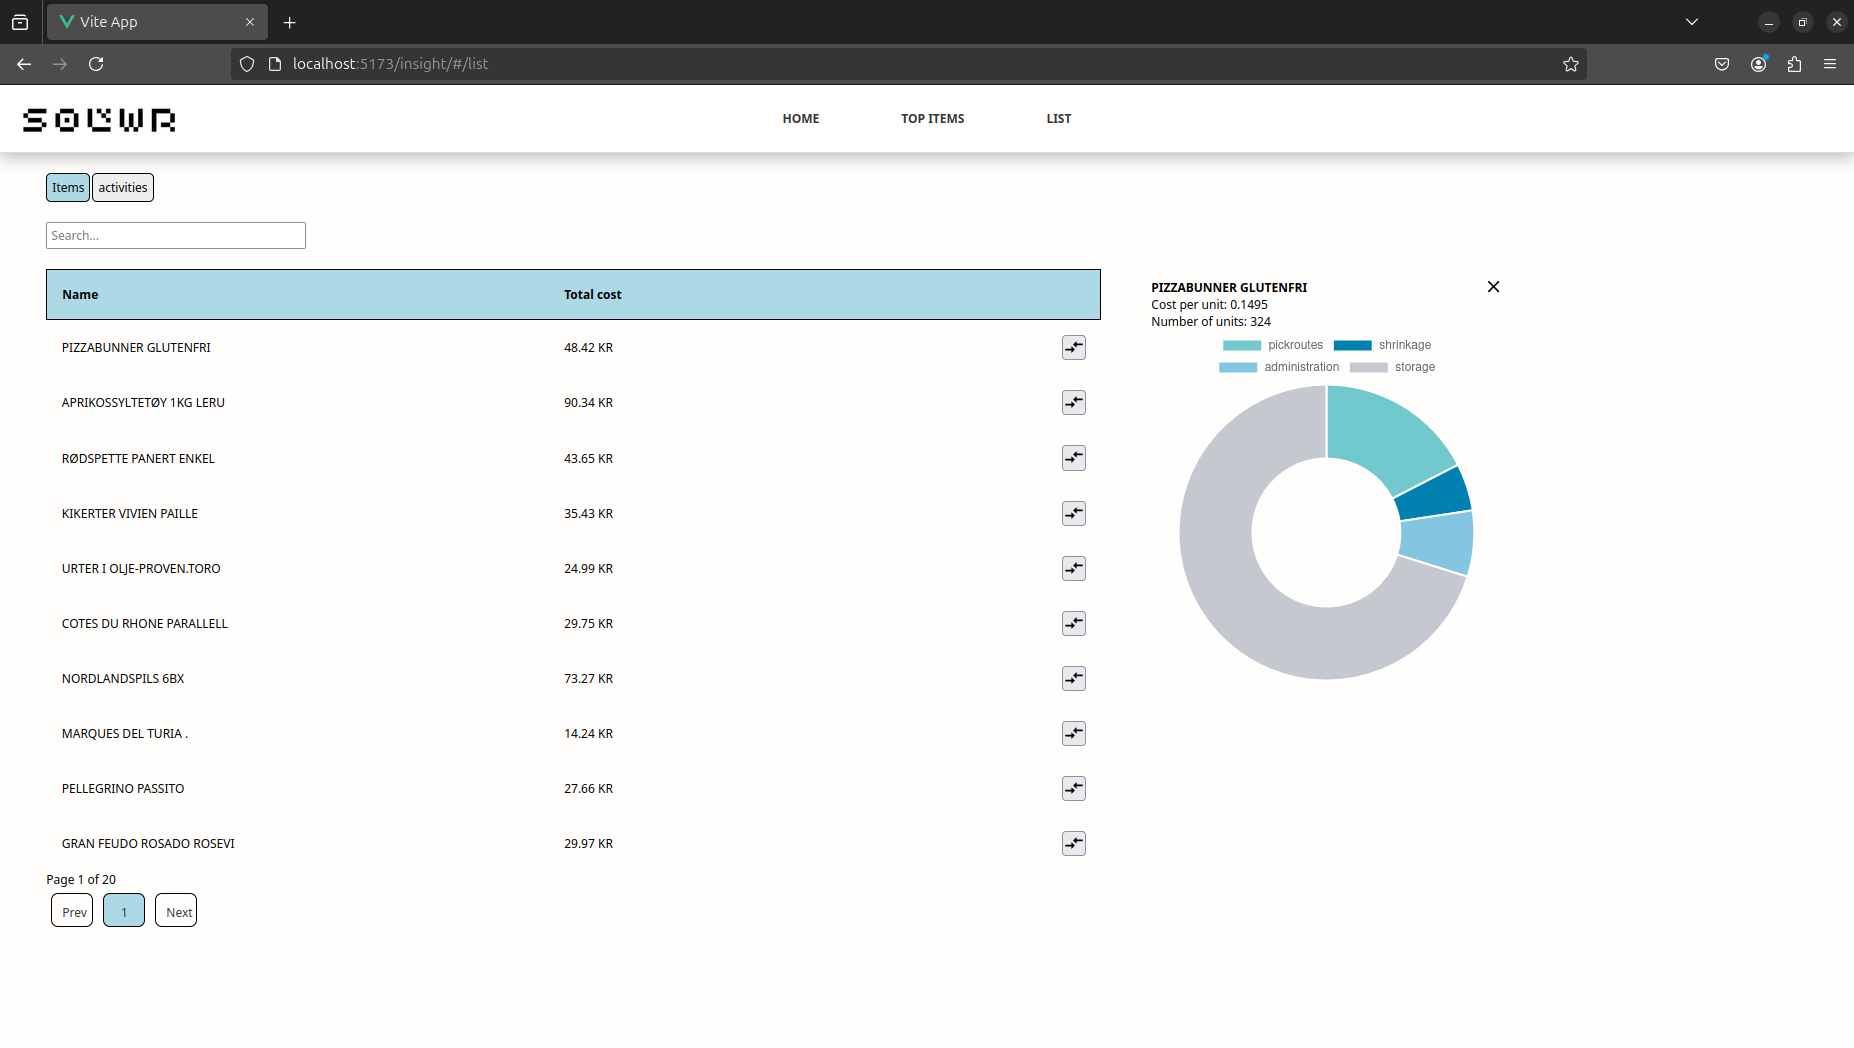
\includegraphics[width=0.45\linewidth]{resources/python app/abc_analysis_python_doughnut.png}}}
    \qquad
    \subfloat[\centering \gls{abc} Analyse \textit{Python} bar-diagram.]{{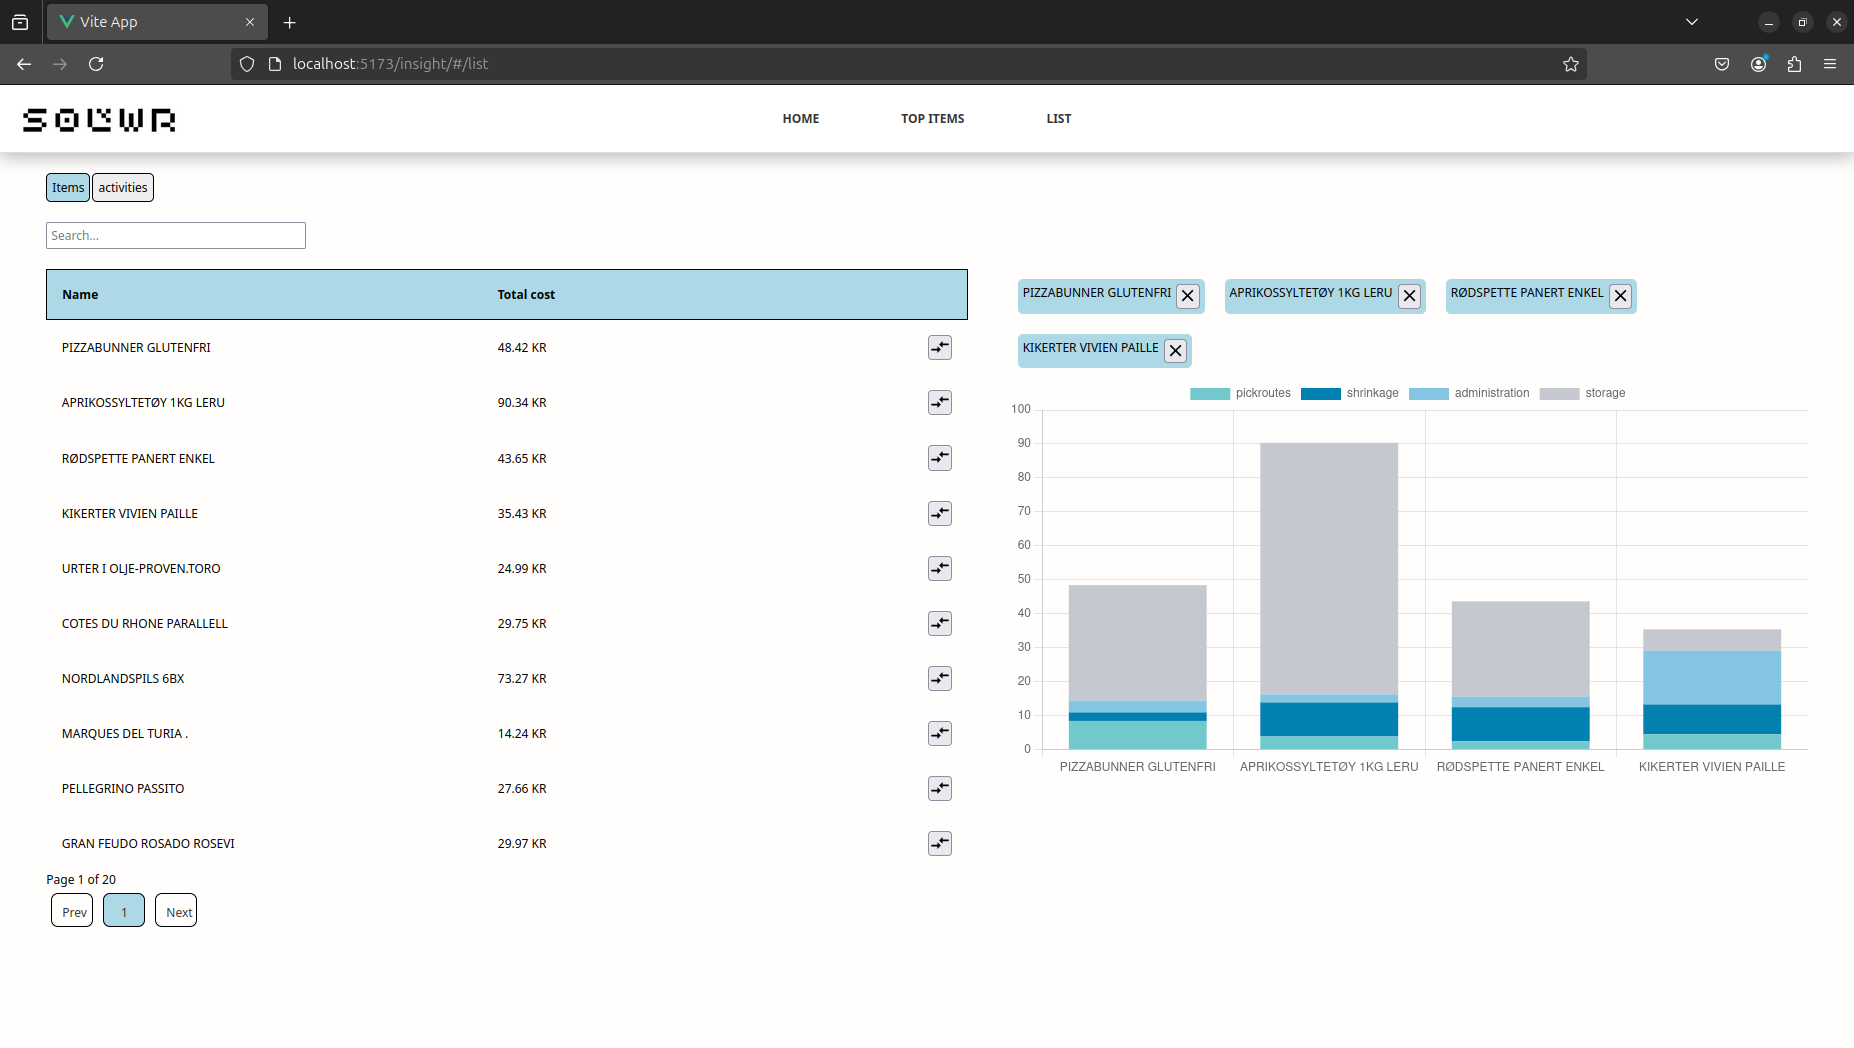
\includegraphics[width=0.45\linewidth]{resources/python app/abc_analysis_python_bar.png}}}
    \caption{\label{fig:abc_analysis_python_application} \acrshort{abc} Anlyse \textit{Python}-applikasjon.}
\end{figure}

\begin{figure}[H]
\centering
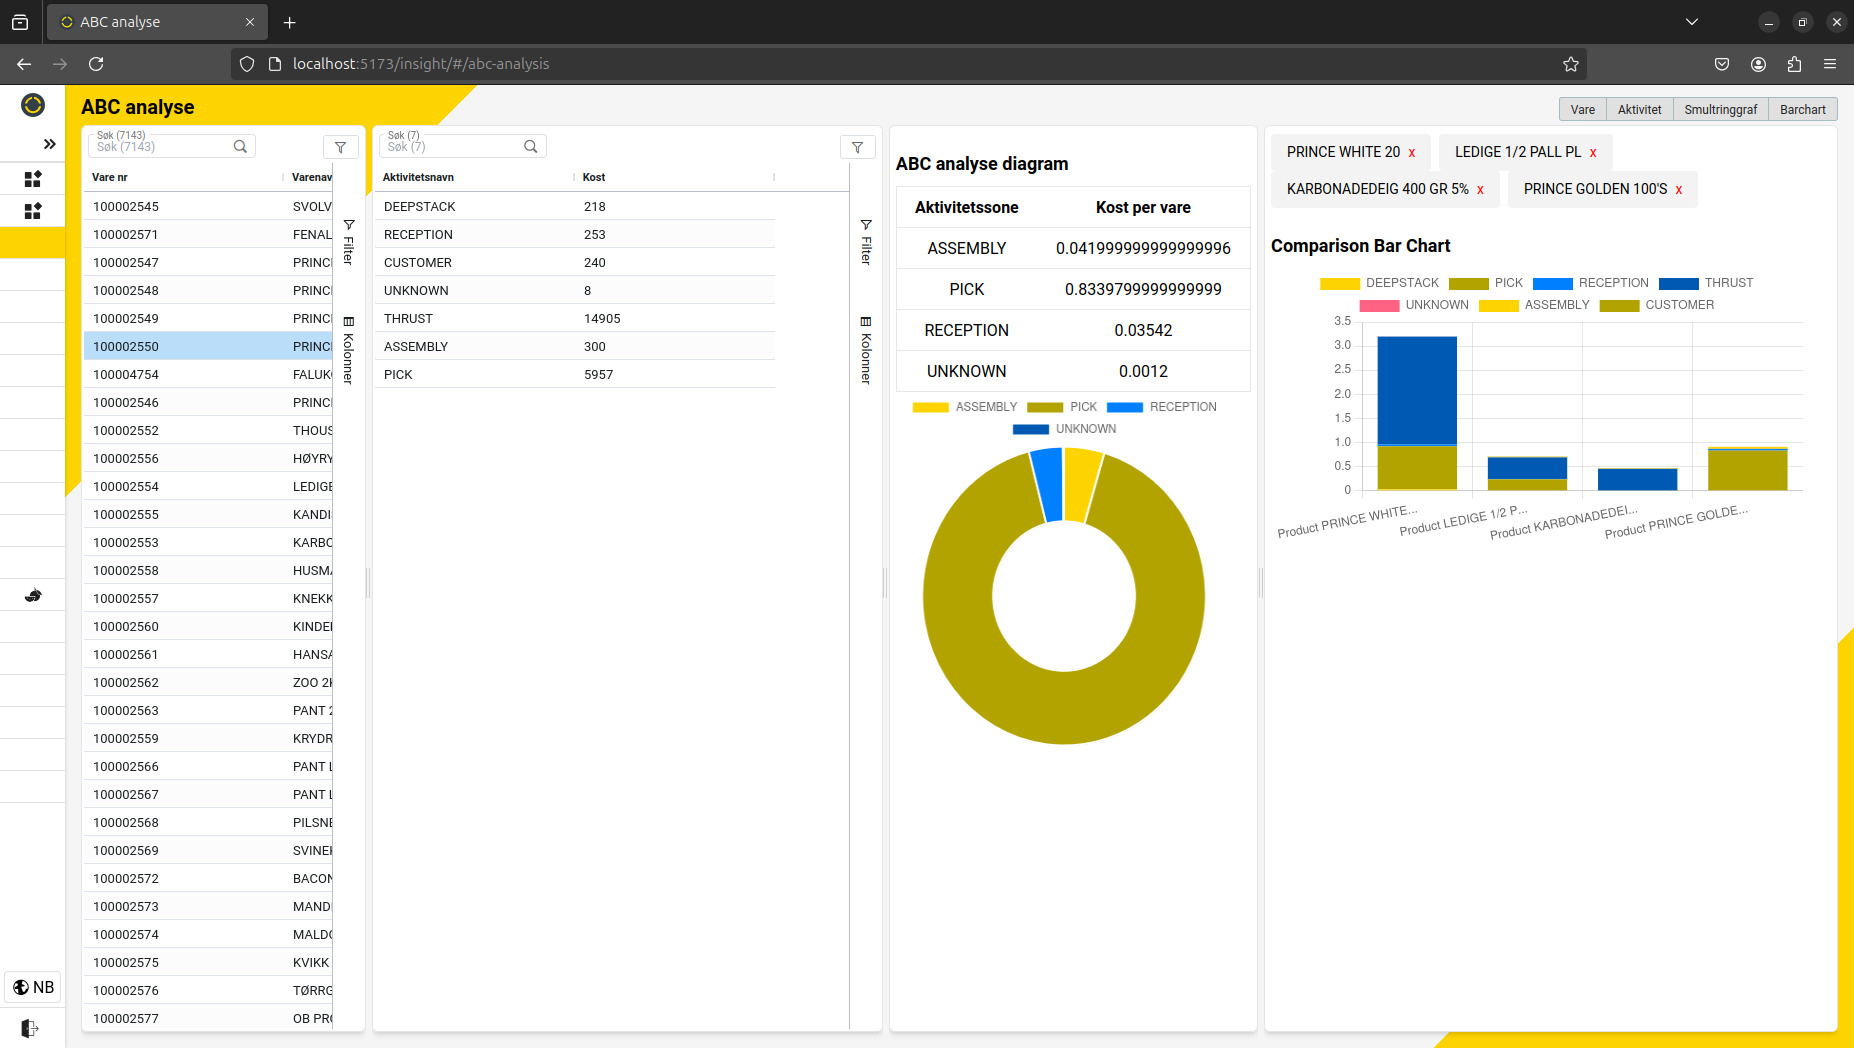
\includegraphics[width=0.8\linewidth]{resources/java app/abc_analysis_trace_insight_bar.png}
\caption{\label{fig:abc_analysis_trace_insight_bar}\gls{trace} | \gls{abc}-analyse modul.}
\end{figure}

% Java-applikasjonen er bygget opp av fire kolonner: \Gls{item}-kolonne, \Gls{aktivitet}s-kolonne, Analyse-kolonne, Sammenlignings-kolonne. Hver av dem har hver sin jobb. \Gls{item}-kolonnen sitt ansvar er å vise brukeren alle varene tilgjenlig å gjøre analyse på. \Gls{aktivitet}s-kolonnen sin jobb er å vise brukeren alle aktiviteter \gls{item}n er i (Koblingen mellom \gls{item} og \gls{aktivitet} er tilfeldig generert). Analyse-kolonnen har ansvar for å vise hvor mye det koster for en \gls{item} å gjøre aktiviteten sin. Sammenlignings-kolonnen skal kunne gi brukeren muligheten til å sammenligne flere \gls{abc}-analyser.

Den nye modulen er strukturert i fire kolonner:
\begin{itemize}
    \item \textbf{\Gls{item}-kolonnen}: Viser alle tilgjengelige varer som kan analyseres.
    \item \textbf{\Gls{aktivitet}s-kolonnen:} Viser aktiviteter knyttet til hver vare. Koblingene er midlertidig tilfeldig generert.
    \item \textbf{Analyse-kolonnen:} Beregner og viser kostnaden for hver vare basert på dens aktiviteter.
    \item \textbf{Sammenlignings-kolonnen:} Lar brukerne sammenligne flere ulike \gls{abc}-analyser.
\end{itemize}

\subsection{Metoder, verktøy og framgangsmåter}

% Metoder som ble brukt av studenten var å ha issues for å holde orden på hva som må bli gjort, hva som jobbes med, og hva som er ferdig. Andre metoder som ble brukt av \gls{rnd} var at alle praktikantene prøvde seg på diverse oppgaver, for å lære om flere områder i kodebasen og ikke bli isolert i sitt eget arbeid, for å så velge den ebste løsningen fra gruppen. Se figur \ref{fig:abc_analysis_trace_insight_bar} for endlig løsning på doughnut diagramet laget av en annen praktikant, og se figur \ref{fig:abc_analysis_trace_insight_my_attempt} for studenten sin løsning. Denne strategien gjør at alle praktikantene lærer om hele modulen, og at man får de beste delene implementert.

% For studenten sine oppgaver ble det brukt diverse teknologier: 
% \begin{itemize}
%     \item \acrlong{vsc} \gls{ide}'en ble brukt for å kode.
%     \item \Gls{git} ble brukt for versjonskontroll av koden.
%     \item DBeaver ble brukt for å designe og lage \gls{sql}-query'er.
%     \item Postman ble brukt for å teste om \gls{api}'ene fungerte som de skulle.
% \end{itemize}

Arbeidet mitt var strukturert ved bruk av at \gls{issue_board} for å organisere oppgaver som må gjøres, pågår, og er fullført. Gruppen praktiserte også en samarbeidsmetode der alle fikk prøve ulike oppgaver i kodebasen. Dette sikret at alle kjente til hele modulen og kunne bidra til den beste løsningen. For eksempel: mens en annen praktikant leverte en ferdig løsning for doughnut-diagrammet, se figur \ref{fig:abc_analysis_trace_insight_bar}, utviklet jeg en alternativ løsning, se figur \ref{fig:abc_analysis_trace_insight_my_attempt}. 

\begin{figure}[H]
\centering
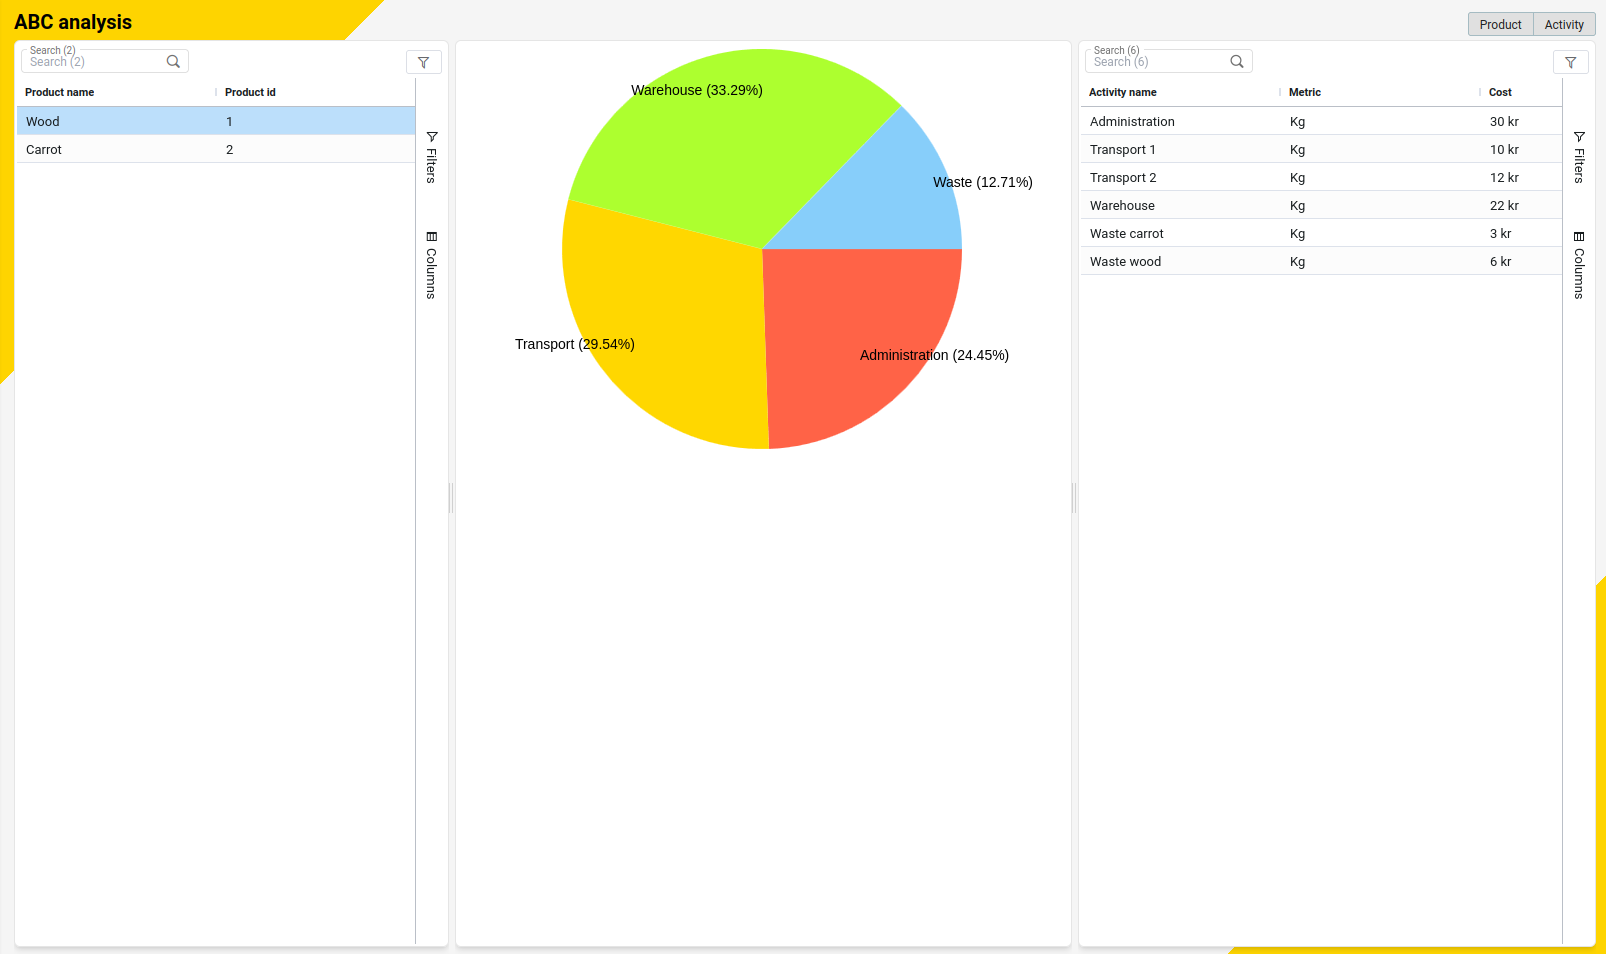
\includegraphics[width=0.8\linewidth]{resources/java app/abc_analysis_trace_insight_my_attempt.png}
\caption{\label{fig:abc_analysis_trace_insight_my_attempt}\gls{trace} | Alternativ doughnut løsning.}
\end{figure}

Verktøy som ble brukt:
\begin{itemize}
    \item \textbf{\gls{vsc}:} For koding.
    \item \textbf{\Gls{git}:} For verjsonskontroll og samarbeid.
    \item \textbf{DBeaver:} For design og teste \gls{sql}-queryer.
    \item \textbf{Postman:} For testing av \gls{api}-funksjonalitet.
\end{itemize}

\subsection{Virksomhetens bruk av resultatene}
% \input{sections/0404 Virksomhetens bruk av resultatene}
% Planen til virksomheten etter praksisen er å videreføre arbeidet over til ansatte hos \textit{Solwr Software}. Ideen var å få praktikanter til å lage skjelettet og vise til 'proof of cencept'. Ettersom dataen som skal brukes i modulen ikke eksisterer, er dette nødt til å bli fikset opp i av bedriften sine utviklere. \\

% Planen for selve modulen er å gi brukerne mulighet til å gjøre \gls{abc}-analyse over produktene deres, dersom det er ønsket. På denne måten får kundene deres en måte å holde oversikt over bruksområder i tillegg til tilgang til de resterende modulene Solwr tilbyr kundene deres.

Arbeidet som ble gjort i praksisperioden, utgjør et \textit{proof of concept} og et rammeverk for videre utvikling. Dette rammeverket vil bli vidreutviklet av virksomhetens interne team i Solwr Software. En viktig del av oppfølgingsarbeidet blir å tilrettelegge for at reelle data kan brukes i applikasjonen.\\
Modulen er planlagt å bli en del av Solwr Software sitt tilbud til sine kunder. Den vil gi brukerne mulighet til å utføre \gls{abc}-analyser av sine produkter.

\subsection{Personer i virksomheten som har gitt rådgiving}

Gjennom praksisperioden mottok jeg verdifull veiledning fra flere nøkkelpersoner:
\begin{itemize}
    \item \textbf{Andrea Tenti:} Veileder med hovedansvar for å forklare den matematiske algoritmen og navigere i databasen.
    \item \textbf{Halvard Øverlien:} Hjalp med systemoppsett og feilsøking, inkludert lokal database og debugging.
    \item \textbf{Mikael Tollefsen:} Teoretisk veiledning om \gls{sql}, og valg av \gls{api}-type samt deres bruk.
    \item \textbf{Sakarias Sæterstøl:} Hjalp med å sette opp Linux-miljøet som ble brukt på arbeidslaptopen.
    \item \textbf{Jon Marius Håkedal:} Løste bitlockerproblem under instalasjon av Linuxmiljøet til arbeidslaptopen.
\end{itemize}